\part{SW02 - HTML}
\section{HTML}
\begin{itemize}[noitemsep,topsep=0pt,leftmargin=*]
    \item Das W3C (World-Wide-Web Consortium) ist für Standardisierung zuständig
    \item Aktuellster fertiger Standard ist Version 5.2 (Dez. 2017)
    \item Zudem wurden verschiedene Themen rund um HTML5 in eigenen Spezifikationen verabschiedet, bzw. sind in der Entwicklung (AAM, HTML Extension Specifications, ARIA,\dots)
\end{itemize}
\subsection{Verstehen wie HTML Informationen strukturiert und wie der Aufbau von HTML Dokumenten ist}
\subsubsection{HTML tags}

\subsection{Wissen wie der \textbf{syntaktische Aufbau} von HTML ist}
\paragraph{$<$head$>$ }
\begin{itemize}[noitemsep,topsep=0pt,leftmargin=*]
    \item Enthält Kopfdaten wie Metainformation, Titel, Stil, Scriptdefinitionen, Adress- und Zielfensterbasis
    \item Ist in jedem HTML Dokument zu finden
    \begin{itemize}[noitemsep,topsep=0pt,leftmargin=*]
        \item Metainformationen werden durch Metatags repräsentiert
        \lstset{language=HTML}
        \begin{lstlisting}
<meta charset="utf-8">
<meta name="author" content="Hans Wurst">
        \end{lstlisting}
        \item Stildefinitionen (CSS - Cascaded Style Sheet) legen Darstellungen fest
        \begin{lstlisting}
<style>
    h1 { color: white; }
    p  { font-wight: bold; }
</style>
        \end{lstlisting}
    \end{itemize}
\end{itemize}

\paragraph{$<$body$>$}
\begin{itemize}[noitemsep,topsep=0pt,leftmargin=*]
    \item HTML \texttt{$<$body$>$} kennzeichnet den Anfang und das Ende des sichbaren Inhalts der WEbseite
    \item Browser zeigen nur den Inhalt zwischen dem öffnenden und schlissenden body-Tag im Browserfenster
    \item Enthält weitere HTML Tags welsche die Information strukturieren, aber auch \textbf{Scripts}, welche an der aufgeführten Stelle ausgeführt werden
    \item Ein HTML-Dokument darf nur einen body-Tag haben
\end{itemize}

\paragraph{Text- und Informations-Strukturierung}
\begin{itemize}[noitemsep,topsep=0pt,leftmargin=*]
    \begin{multicols}{2}
        \item Absatz
        \item Zeilenumbruch
        \item Vorformatierung
        \item Überschriften
        \item Waagrechte Linien
        \item Container
        \columnbreak
        \begin{lstlisting}
<p>..</p>
<br />
<pre>..</pre>
<h1>..</h1> bis <h6>..</h6>
<hr />
<div>..</div> oder <span>..</span>
        \end{lstlisting}
    \end{multicols}
    \item Sind alles \textbf{Blockelemente}, das heisst, ein neuer Absatz (Zeilenumbruch) wird eingeleitet
\end{itemize}

\paragraph{Verfügungen (Hypertext-Referenzen)}
\begin{itemize}[noitemsep,topsep=0pt,leftmargin=*]
    \item Link
    \begin{lstlisting}
<a href="pfad/datei">Linktext</a>
    \end{lstlisting}
    \item Sowohl lokal als auch ins Internet möglich
    \begin{lstlisting}
<a href="/index.html">Home</a>
<a href="http://www.hslu.ch">Gehe zu HSLU</a>
    \end{lstlisting}

    \item Mail-Links
    \begin{lstlisting}
<a href="mailto:hans@muster.ch">Mail schreiben</a>
    \end{lstlisting}
    \begin{itemize}[noitemsep,topsep=0pt,leftmargin=*]
        \item Sollte vermieden werden, da Spambots diese automatisiert auslesen
    \end{itemize}
        \item Interne Verknüpfung mittels Anker
    \begin{lstlisting}
<a href="#Kapitel1">Kapitel 1</a>
    \end{lstlisting}
    \item als Ziel dieses Links
    \begin{lstlisting}
<p id="Kapitel1">Kapitel 1</p>
    \end{lstlisting}
    \item Öffnen im neuen Fenster
    \begin{lstlisting}
<a href="adresse" target="_blank">Adresse</a>
    \end{lstlisting}
\end{itemize}

\paragraph{Grafiken}
\begin{itemize}[noitemsep,topsep=0pt,leftmargin=*]
    \item Grafikformate gif, jpg, png, \dots
    \item Einbinden mit
    \begin{lstlisting}
<img src="pfad/bildname" alt="Beschreibung" />
    \end{lstlisting}
    \item alt-Attribut verwenden spezielle Browser (Barrierefreiheit) oder Suchmaschinen (z.B. Google Bildersuche), unbedingt angeben
    \item Anzeigegrösse veränderbar mit Attributen \texttt{width} und \texttt{height}
    \item Rahmen: border="'1px"' %TODO
    \item Als Hintergrund der Seite
    \begin{lstlisting}
<body background="bildname">
    \end{lstlisting}
\end{itemize}

\paragraph{Klickbare Grafiken: Imagemaps}
\begin{enumerate}[noitemsep,topsep=0pt,leftmargin=*]
    \item Definition des Bildes
    \begin{lstlisting}
<map name="karte">
    <area shape="circle" coords="50,50,45" href="Ziel.html" alt="Reiseziel" />
</map>
    \end{lstlisting}
    \begin{itemize}[noitemsep,topsep=0pt,leftmargin=*]
        \item Wird häufig zu Navigationszwecken verwendet
    \end{itemize}
\end{enumerate}

\paragraph{Beispiel}Imagemap-Code
\begin{lstlisting}
<body>
    ...
    <img src="transmap.gif" alt="list of stations" usemap="#transmap">
    <map name="transmap">
        <area shape="rect" coords="59,390,172,441" href="#ACACIA" />
        <area shape="rect" coords="280,21,390,63" href="#ALMOND" />
        <area shape="rect" coords="135,52,243,124" href="#APPLE" />
        <area shape="rect" coords="141,235,189,284" href="#ASH" />
        <area shape="rect" coords="110,336,205,388" href="#BEECH" />
        <area shape="rect" coords="152,289,236,334" href="#BIRCH" />
        <area shape="rect" coords="330,231,402,288" href="#CHERRY" />
        ...
    </map>
    ...
    <a name="ACACIA">Acacia</a><img src="red.gif" alt="Red Line" />
    ...
    <a name="ALMOND">Almond</a><img src="yellow.gif" alt="Yellow Line" />
    ...
</body>
\end{lstlisting}

\paragraph{Metatags}
\begin{itemize}[noitemsep,topsep=0pt,leftmargin=*]
    \item Werden nicht zur Gestaltung sondern \textbf{zur Beschreibung des Inhalts} verwendet (daher der Name: Meta-Information)
    \item Werden im \texttt{head} Bereich eingefügt
    \item Aufbau:
    \begin{lstlisting}
<meta name="Schlüsselwort" content="Inhalt">
    \end{lstlisting}
    \item Die wichtigsten Metatags
    \begin{itemize}[noitemsep,topsep=0pt,leftmargin=*]
        \item keywords
        \item description
        \item language
        \item page-topic (Thema für Suchmaschinen und Kataloge)
        \item audience (Zielgruppe in Suchmaschinen und Katalogen)
        \item robots (zur Linkverfolgung)
        \item refresh (und expires $\rightarrow$Ablaufdatum)
        \item copyright
    \end{itemize}
\end{itemize}

\paragraph{Sonderzeichen}
\begin{itemize}[noitemsep,topsep=0pt,leftmargin=*]
    \item Damit Sonderzeichen korrekt dargestellt werden, muss das charset metatag korrekt gesetzt sein
    \begin{lstlisting}
<meta charset="utf8">
<meta charset="iso-8859-1">
    \end{lstlisting}
    \item Eine Alternative ist die Zeichen speziell zu kodieren:\\
    Beispiel: aus \textbf{ü} wird \textbf{\&uuml;}
    \item Dies ist auch notwendig bei Zeichen, welche mit dem HTML-Markup kollidieren:\\
    \& zu \&amp;, $<$ zu \&lt;, $>$ zu \&gt;, %TODO "` zu \&quot;, \quote zu \&#39;
\end{itemize}

\paragraph{Masseinheiten}
\begin{itemize}[noitemsep,topsep=0pt,leftmargin=*]
    \item Verwendet in Attributen zur Bestimmung der Dimensionen verschiederer Elemente wie Bilder, Schriften, Ränder, Abstände
    \item Die wichtigsten Einheiten sind:
    \begin{itemize}[noitemsep,topsep=0pt,leftmargin=*]
        \item pt: Punkt, \textbf{absolute} Angabe, 1 Punkt entspricht 1/72 Inches
        \item in: Inch, \textbf{absolute} Angabe, 1 Inch enspricht 2.54cm
        \item mm: Millimeter, \textbf{absolute} Angabe
        \item px: Pixel, \textbf{absolute/relative} Angabe Abhängig von der \textbf{Pixeldichte} des Ausgabegeräts
        \item em: M, \textbf{relative} Angabe, auf die Schriftgrösse des Elements bezogen (mit Ausnahmen)
        \item \%: Prozent, \textbf{relative} Angabe, je nach CSS-Eigenschaft relativ zur elementeigenen Grösse, oder zu der des Elternelements, oder zu einem allgemeineren Kontext
    \end{itemize}
\end{itemize}

\paragraph{Farben}
\begin{itemize}[noitemsep,topsep=0pt,leftmargin=*]
    \item Farben werden aus den RGB-Wertangaben gebildet
    \item Beispiel: \#FF0000 ist rot, \#00FF00 ist grün, \#0000FF ist blau
    \item Werte werden in hexadezimaler Form angegeben
    \item Werte von \#00 bis \#FF (255) sind möglich
    \item Einige Farben sind per Namen in der DTD (Document-Type-Definition) definiert:
    \begin{align*}
&\text{Black}&      &=\text{\#00000}&   &\text{Green}&   &=\text{\#008000}\\
&\text{Silver}&     &=\text{\#C0C0C0}&  &\text{Lime}&    &=\text{\#00FF00}\\
&\text{Gray}&       &=\text{\#808080}&  &\text{Olive}&   &=\text{\#808000}\\
&\text{White}&      &=\text{\#FFFFFF}&   &\text{Yellow}&  &=\text{\#FFFF00}\\
&\text{Maroon}&     &=\text{\#800000}&   &\text{Navy}&    &=\text{\#000080}\\
&\text{Red}&        &=\text{\#FF0000}&   &\text{Blue}&    &=\text{\#0000FF}\\
&\text{Purple}&     &=\text{\#800080}&   &\text{Teal}&    &=\text{\#008080}\\
&\text{Fuchsia}&    &=\text{\#FF00FF}&   &\text{Aqua}&    &=\text{\#00FFFF}\\
    \end{align*}
\end{itemize}

\subsubsection{Struktur von Webseiten - Elemente}
\begin{figure}[H]
    \begin{center}
    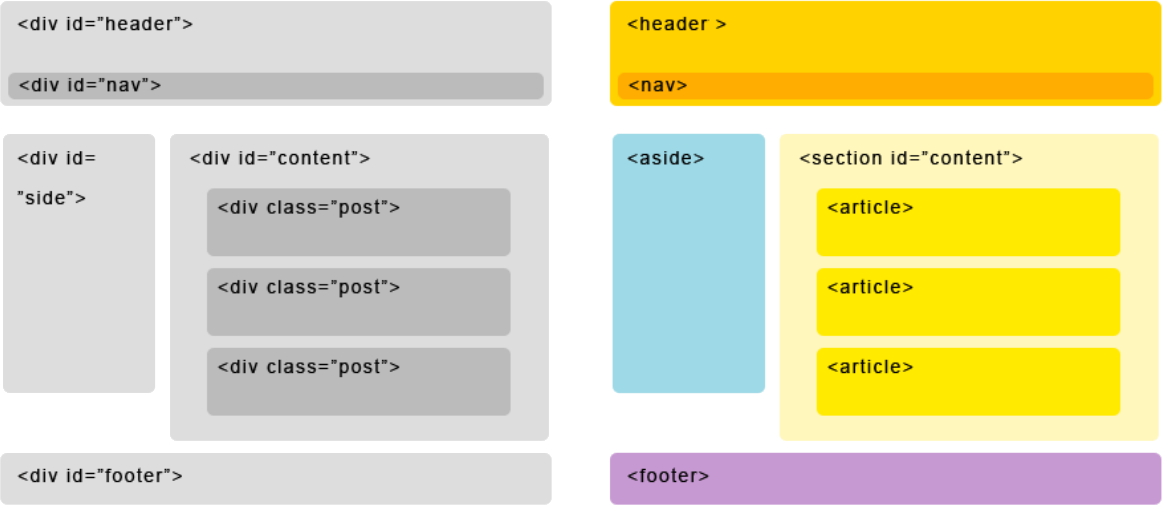
\includegraphics[width=14cm]{images/struktur.png}
    \caption{Strukturbeispiel von Webseiten}
    \label{strukturHTML}
    \end{center}
\end{figure}

\paragraph{$<$header$>$}
\begin{itemize}[noitemsep,topsep=0pt,leftmargin=*]
    \item enthält sichtbaren Kopfbereich einer Webseite
    \item Gruppierung einleitender Inhalte (Firmenlogos, Motto, Navigationslinks)
\end{itemize}

\paragraph{$<$footer$>$}
\begin{itemize}[noitemsep,topsep=0pt,leftmargin=*]
    \item enthält Informationen, die in Webseiten am Ende stehen: Autor, Hinweise zum Urheberrecht, ein Link zum Impressum
    \item Position ist nicht notwendigerweise am unteren Rand\\
    $\rightarrow$bei Blogeinträgen steht der footer oft neben dem Text
\end{itemize}

\paragraph{$<$article$>$}
\begin{itemize}[noitemsep,topsep=0pt,leftmargin=*]
    \item stellt in sich geschlossene Abschnitte eines Dokuments dar\\
    $\rightarrow$vergleichbar mit einem Zeitungsartikel\\
    $\rightarrow$innterhalb von article-Elementen weitere strukturierende Elemente wie header, section oder footer
\end{itemize}

\paragraph{$<$section$>$}
\begin{itemize}[noitemsep,topsep=0pt,leftmargin=*]
    \item enthält eine thematische Gruppierung von Inhalten typischerweise mit einer Überschrift
    \item dient dazu, den Inhalt oder auch einen article in semantische Abschnitte zu gliedern
\end{itemize}

\paragraph{$<$nav$>$}
\begin{itemize}[noitemsep,topsep=0pt,leftmargin=*]
    \item umschliesst insbesondere Navigationsleisten
    \item kann neben einer ungeordneten Liste mit den Verweisen auch eine Überschrift oder ähnliches enthalten
\end{itemize}

\paragraph{$<$aside$>$}
\begin{itemize}[noitemsep,topsep=0pt,leftmargin=*]
    \item umschliesst Abschnitte einer Seite, deren Inhalt nur in einem indirekten Zusammenhang mit dem umgebenden Inhalt stehen
    \item Beispiele: Randbemerkungen, Fussnoten oder Links zu weitergehenden Webseiten
\end{itemize}


\subsection{Kennen von \textbf{geeigneten Werkzeugen} für das Erstellen, Bearbeiten, Darstellen, Validieren etc. von HTML Dokumenten}

\subsection{Wissen um geeignete \textbf{Quellen und Referenzen} im Internet}
